\textnormal{
The data from a common source file is run through the Huffman source coding algorithm and the encoded tree is generated. This encoded tree is shared with the receiver for decompression. Now we will be using the same encoded tree for compressing data files of similar type.The decompressing algorithm for the file will remain the same except that we will be using the same priority queue. Moreover, we will have more compression of the header file as we will not have to send the Huffman coding tree. The following is the algorithm and flow diagram of the proposed project-
\\*
Algorithm:
\begin{enumerate}
\item{Sort source outputs in decreasing order of their probabilities/frequencies}
\item{Implement the priority queue for each charcater with their frequencies}
\item{Merge the two least probable/frequent characters/outputs from the priority into a single output by adding their corresponding probabilities/frequencies}
\item{Repeat the above step until we are left with 2 characters.The sum of probability of these two characters should be 1 and sum of their frequecies will be equal to the total number of characters in the data source}
\item{Arbitrarily assign 0 and 1 as code word for the two remaining characters/outputs from step 4}
\item{If an output is the result of the merger of two outputs in a preceding step, append the current code word with a 0 and a 1 to obtain the code word for the preceding outputs; then, repeat Step 6. If no output is preceded by the output in current step, then stop.}
\item{This will result in a Huffman coding tree which will be used to compress the data}
\item{Now use the same Huffman coding tree from step 7 to compress other data fies of similar type}
\item{All the binary files are decompressed using the same huffman coding tree generated on step 7}
\end{enumerate}
Flow Diagram:
\\*
\begin{figure}[!h]
    \centering
    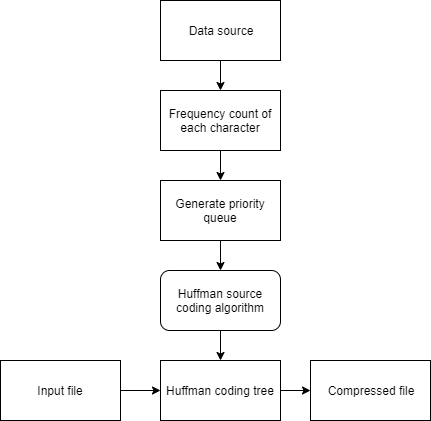
\includegraphics[width=90mm,scale=0.5]{Data Flow.png}
    \caption{Data Flow}
\end{figure}
\\*
High Level Pseudo Code System Description:
\\
procedure Huffman(f)
\begin{itemize}
  \item[] Input: An array f[1...n] of frequencies
  \item[] Output: An encoding tree with n leaves
  \item[] Let H be a priority queue of integers, ordered by f
  \item[] for i = 1 to n: 
  \item[]\makebox[0.5cm][l]{ } insert(H; i)
  \item[]for k = n + 1 to 2n - 1:
  \item[]\makebox[0.5cm][l]{ } i = deletemin(H); j = deletemin(H) 
  \item[]\makebox[0.5cm][l]{ } create a node numbered k with children i, j
  \item[]\makebox[0.5cm][l]{ } left[k] <- i
  \item[]\makebox[0.5cm][l]{ } right[k] <-j
  \item[]\makebox[0.5cm][l]{ } f[k] = f[i] + f[j]
  \item[]\makebox[0.5cm][l]{ } insert(H, k)
  \item[] return k
\end{itemize}
Here k represents the root of the Huffman coding tree with n leaves. Now we will use the same tree for compressing all data files of similar types.
\\
Data Structures:
\begin{itemize}
\item {Python Dictionary: The python dictionary stores data in a similar way as the regular dictionary. It has keys which are associated with corresponding values and these values can be referenced using the keys.}
\item {Priority Queue: A priority queue is stored in form of array/list and implemented using heaps. New values are inserted at the back and removal of values is done from the front. However, the priority of the elements is always maintained at the front and the element with the lowest priority is moved to the back.}
\end{itemize}
Complexity Analysis:
\\
Running time complexity - The conventional Huffman coding algorithm involves the calculation of frequencies for each character. For this step we need to read the entire data source once which will take time of O(n). The other time consuming step would be the deletemin and insert operations on the priority queue. Each iteration on priority queue takes O(log n). There are n iterations, one for each data point, so the overall running time complexity will be O(nlog n). In our algorithm, the first file for compression will take O(nlog n) running time, but for the subsequent files we will neithe calculate frequencies nor maintain the priority queue. Thus each character will be read from the data source and converted into binary sequences. This will take linear time to code the data.
\\
Space Complexity - The conventional algorithm requires space to maintain the priority queue for each data file. In our case this space is fixed and the stored priority queue does not change.
\\*
Constraints:
\\
It is important to note that the above proposed algorithm only works for compressing files of similar types. This is because we are using the same Hufmann coding tree generated from one common source file. While compressing a new file, if we find a new character that is not present in the Huffman coding tree then our compression algorithm will fail. So we have to be careful while choosing the data source for generating the Huffman coding tree. This data source should have all the characters that we will encounter while compressing and also the probability distribution of characters should be similar among the various input files.
\\
Timeline for the project:
\begin{itemize} 
\item{October 28th to November 2nd: Complete the description of the project} 
\item{November 2nd to November 4th: Draft a pseudo code and prepare a flow diagram for the project}
\item{November 4th to November 6th: Identifying data sets for implementing Huffman coding algorithm}
\item{November 7th to November 10th: Implementing the Huffman coding algorithm in python}
\item{November 10th to November 15th: Generate the Intermidiate report with the results so far}
\item{November 15th to November 17th: Implementing the Huffman coding algorithm on similar data sets}
\item{November 18th to November 20th: Analyse the time and space complexity and compare the compression ratios for various data sets}
\item{November 21st to November 23rd: Tabulate the results}
\item{November 24th to November 25th: Identify future extensions}
\item{November 25th to November 27th: Prepare the final report and presentation ppt, present to TA.}
\end{itemize}
Division of labor:
\begin{itemize}
\item {Praneeth: Implementation of the Huffman coding algorithm and making the presentation ppt}
\item {Naveen: Literature Review, tabulating the results and generating the reports}
\end{itemize}
}





